% FAS2GraphTheoryTikZ-001.tex
% Asset ID: FAS2GraphTheoryTikZ-001
% Unit: FAS2 Further AS 2 Applied Mathematics
% Topic Code: FAS2-GRAPH
% Topic Name: Graph theory
% Topic ID: FAS2GraphTheory
% Related lesson file: FAS2_graph_theory_lesson.md
% Related lesson section: Section 9 Visual Asset Integration; Worked Examples 1 to 3
% Source: Uploaded teacher transcript and lesson PDF for Chapter 2 Graphs & Networks
% Purpose: Provide a precise weighted graph diagram for graph, network, subgraph and degree examples.

\documentclass[tikz,border=8pt]{standalone}
\usepackage{tikz}
\usetikzlibrary{calc,positioning}
\definecolor{Canvas}{HTML}{FAF9F6}
\definecolor{Ivory}{HTML}{FFFFF0}
\definecolor{Line}{HTML}{2C2C2E}
\definecolor{Divider}{HTML}{E5E5EA}
\definecolor{Gold}{HTML}{C5A059}
\definecolor{SoftGold}{HTML}{D4AF37}
\definecolor{Blush}{HTML}{FBEFEF}

\begin{document}
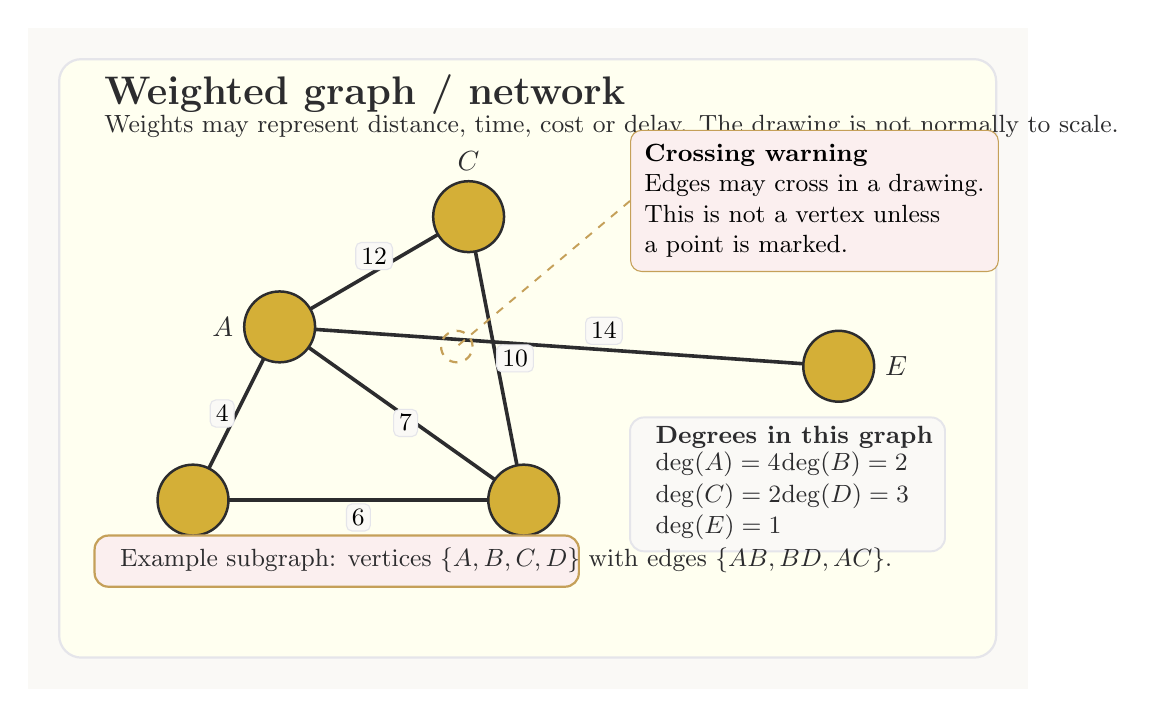
\begin{tikzpicture}[
  vertex/.style={circle,draw=Line,fill=SoftGold,line width=0.9pt,minimum size=9mm,inner sep=0pt,font=\bfseries},
  edge/.style={draw=Line,line width=1.3pt,line cap=round},
  weight/.style={fill=Canvas,draw=Divider,rounded corners=2pt,inner sep=2pt,font=\small},
  note/.style={fill=Blush,draw=Gold,rounded corners=4pt,align=left,inner sep=5pt,font=\small}
]
\fill[Canvas] (-1.2,-1.2) rectangle (11.5,7.2);
\draw[draw=Divider,fill=Ivory,rounded corners=8pt,line width=0.8pt] (-0.8,-0.8) rectangle (11.1,6.8);
\node[anchor=west,font=\Large\bfseries,text=Line] at (-0.35,6.35) {Weighted graph / network};
\node[anchor=west,font=\small,text=Line] at (-0.35,5.95) {Weights may represent distance, time, cost or delay. The drawing is not normally to scale.};
\coordinate (A) at (2.0,3.4); \coordinate (B) at (0.9,1.2); \coordinate (C) at (4.4,4.8); \coordinate (D) at (5.1,1.2); \coordinate (E) at (9.1,2.9);
\draw[edge] (A)--(B); \draw[edge] (A)--(C); \draw[edge] (A)--(D); \draw[edge] (B)--(D); \draw[edge] (C)--(D); \draw[edge] (A)--(E);
\node[weight] at ($(A)!0.50!(B)+(-0.18,0)$) {$4$};
\node[weight] at ($(A)!0.50!(C)+(0,0.20)$) {$12$};
\node[weight] at ($(A)!0.50!(D)+(0.05,-0.12)$) {$7$};
\node[weight] at ($(B)!0.50!(D)+(0,-0.22)$) {$6$};
\node[weight] at ($(C)!0.50!(D)+(0.24,0)$) {$10$};
\node[weight] at ($(A)!0.58!(E)+(0,0.24)$) {$14$};
\node[vertex,label={[text=Line,font=\bfseries]left:$A$}] at (A) {};
\node[vertex,label={[text=Line,font=\bfseries]below:$B$}] at (B) {};
\node[vertex,label={[text=Line,font=\bfseries]above:$C$}] at (C) {};
\node[vertex,label={[text=Line,font=\bfseries]below:$D$}] at (D) {};
\node[vertex,label={[text=Line,font=\bfseries]right:$E$}] at (E) {};
\coordinate (X) at (4.25,3.15);
\draw[draw=Gold,dashed,line width=0.8pt] (X) circle (0.20);
\node[note,anchor=west] (crossnote) at (6.45,5.0) {\textbf{Crossing warning}\\Edges may cross in a drawing.\\This is not a vertex unless\\a point is marked.};
\draw[draw=Gold,dashed,line width=0.7pt] (crossnote.west)--(X);
\draw[draw=Divider,fill=Canvas,rounded corners=5pt,line width=0.7pt] (6.45,0.55) rectangle (10.45,2.25);
\node[anchor=west,font=\small\bfseries,text=Line] at (6.65,2.00) {Degrees in this graph};
\node[anchor=west,font=\small,text=Line] at (6.65,1.65) {$\deg(A)=4$};
\node[anchor=west,font=\small,text=Line] at (8.25,1.65) {$\deg(B)=2$};
\node[anchor=west,font=\small,text=Line] at (6.65,1.25) {$\deg(C)=2$};
\node[anchor=west,font=\small,text=Line] at (8.25,1.25) {$\deg(D)=3$};
\node[anchor=west,font=\small,text=Line] at (6.65,0.85) {$\deg(E)=1$};
\draw[draw=Gold,rounded corners=5pt,line width=0.8pt,fill=Blush] (-0.35,0.1) rectangle (5.8,0.75);
\node[anchor=west,font=\small,text=Line] at (-0.15,0.43) {Example subgraph: vertices $\{A,B,C,D\}$ with edges $\{AB,BD,AC\}$.};
\end{tikzpicture}
\end{document}
